% Gradient Info
\tikzset {_q0xe4a8ap/.code = {\pgfsetadditionalshadetransform{ \pgftransformshift{\pgfpoint{0 bp } { 0 bp }  }  \pgftransformscale{1 }  }}}
\pgfdeclareradialshading{_bttg32ha4}{\pgfpoint{0bp}{0bp}}{rgb(0bp)=(0.97,0.91,0.11);
	rgb(0bp)=(0.97,0.91,0.11);
	rgb(25bp)=(0.97,0.91,0.11);
	rgb(400bp)=(0.97,0.91,0.11)}
\tikzset{_2y6lizc3m/.code = {\pgfsetadditionalshadetransform{\pgftransformshift{\pgfpoint{0 bp } { 0 bp }  }  \pgftransformscale{1 } }}}
\pgfdeclareradialshading{_cmven2zpf} { \pgfpoint{0bp} {0bp}} {color(0bp)=(transparent!96);
	color(0bp)=(transparent!96);
	color(25bp)=(transparent!69);
	color(400bp)=(transparent!69)} 
\pgfdeclarefading{_uld39de5b}{\tikz \fill[shading=_cmven2zpf,_2y6lizc3m] (0,0) rectangle (50bp,50bp); } 
\tikzset{every picture/.style={line width=0.75pt}} %set default line width to 0.75pt
       

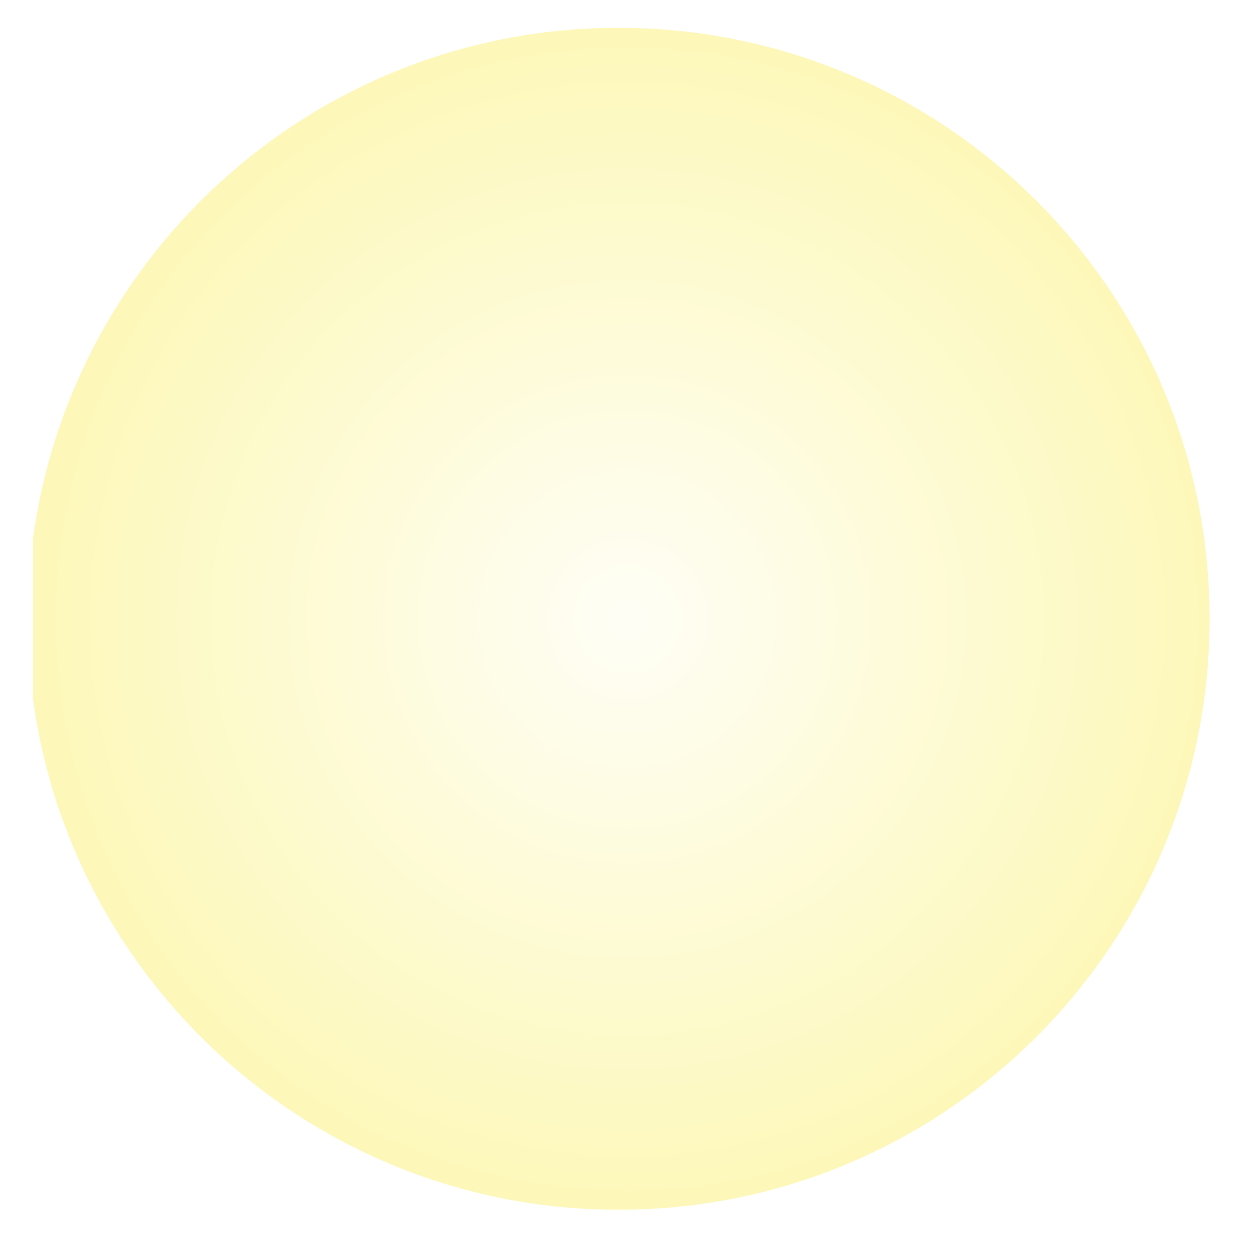
\begin{tikzpicture}[x=0.75pt,y=0.75pt,yscale=-1,xscale=1]


%Shape: Circle [id:dp12550546475470603] 
\path  [shading=_bttg32ha4,_q0xe4a8ap,path fading= _uld39de5b ,fading transform={xshift=2}] (53,302.75) .. controls (53,145.49) and (180.49,18) .. (337.75,18) .. controls (495.01,18) and (622.5,145.49) .. (622.5,302.75) .. controls (622.5,460.01) and (495.01,587.5) .. (337.75,587.5) .. controls (180.49,587.5) and (53,460.01) .. (53,302.75) -- cycle ;

 % for fading 
%\draw  [dash pattern={on 0.84pt off 2.51pt}] (53,302.75) .. controls (53,145.49) and (180.49,18) .. (337.75,18) .. controls (495.01,18) and (622.5,145.49) .. (622.5,302.75) .. controls (622.5,460.01) and (495.01,587.5) .. (337.75,587.5) .. controls (180.49,587.5) and (53,460.01) .. (53,302.75) -- cycle ; % for border 





\end{tikzpicture}

